\clearpage
\setcounter{page}{1}
\maketitlesupplementary


% The supplementary materials provide additional analysis to enrich the main paper, along with further results and insights.
% This document is organized as follows: In Section~\ref{sec:sup_sourcecode} we provide the source code and demo resources, with implementation details in Section~\ref{sec:sup_sourcecode_details}. Section~\ref{sec:sup_results} presents additional results, including a time and memory analysis (Section~\ref{sec:sup_results_time}), guidance ablations (Section~\ref{sub:sup_results_ablation}), and a reconstruction evaluation (Section~\ref{sec:sup_reconstruction}). Finally, Sections~\ref{sec:sup_limitations_structure} and~\ref{sec:sup_limitations_failure} discuss limitations regarding structure preservation and failure cases.


The supplementary materials provide additional analysis to enrich the main paper, along with further results and insights. This document is structured as follows: Section~\ref{sec:sup_sourcecode} contains the source code and demo resources, with implementation information provided in Section~\ref{sec:sup_sourcecode_details}. Section~\ref{sec:sup_results} presents additional experimental outcomes including time and memory requirements (Section~\ref{sec:sup_results_time}), guidance ablations (Section~\ref{sub:sup_results_ablation}), and an evaluation of reconstruction performance (Section~\ref{sec:sup_reconstruction}). Finally, Sections~\ref{sec:sup_limitations_structure} and~\ref{sec:sup_limitations_failure} discuss limitations regarding structure preservation and failure cases.









\section{Source Code}
\label{sec:sup_sourcecode}
% The source code, the scripts to replicate the experiments, as well as a web demo both off-line (\textit{i.e.,} the Gradio app) and on-line (\textit{i.e.,} Huggingface demo) are available at \codeurl{}.The PIE-Bench images corresponding to the quantitative results in Tables \ref{tab:ablation_piebench}, \ref{tab:comparison_piebench}, and \ref{tab:user_study} of the main paper are available as well in a PNG file with all the parameters as metadata so further analysis can be performed on it if needed.

The source code, scripts for replicating the experiments, and a web demo (including an offline version via the Gradio app and an online version hosted on Hugging Face) are available at \codeurl{}. Additionally, the PIE-Bench and MagicBrush images used for the quantitative results in Tables \ref{tab:ablation_piebench}, \ref{tab:comparison_piebench}, and \ref{tab:user_study} of the main paper are also accessible. These images are provided in PNG format, with all editing parameters embedded as metadata, facilitating further independent analysis.

\subsection{Implementation Details}
\label{sec:sup_sourcecode_details}

In our preliminary analysis, best results for $512 \times 512$ images were achieved with $32 \times 32$ self-attention maps and $16 \times 16$ cross-attention maps, particularly from the second and third encoder blocks of the U-Net respectively and the corresponding upsampling block, similar to \cite{hertz2023prompt}. For $ 768 \times 768 $ images, the best results were obtained with $ 24 \times 24 $ self-attention and cross-attention maps, specifically from the third block. Additionally, our code supports FP16 computation, including gradient calculation, which significantly reduces time and memory consumption. To prevent gradients from becoming zero in half-precision floating-point arithmetic, the loss term is scaled by a factor of 500 prior to gradient computation, with the weighting factor $\lambda$ applied afterward (Sec.~\ref{sec:self_attention_guidance}).



\section{Additional Results}
\label{sec:sup_results}

\subsection{Inference time and memory comparison}
\label{sec:sup_results_time}

% \begin{table*}[htbp]
%     \centering
%       \renewcommand\arraystretch{0.9}
%       \setlength{\tabcolsep}{0.3mm}{
%     \begin{threeparttable}
%     \begin{tabular}{c|c|cccc|cc}
%     \toprule
%     \toprule
%           & \textbf{Structure}          & \multicolumn{4}{c|}{\textbf{Background Preservation}} & \multicolumn{2}{c}{\textbf{CLIP Similariy}} \\ \midrule
%     \textbf{Method}            & \textbf{Distance}$_{^{\times 10^3}}$ $\downarrow$ & \textbf{PSNR} $\uparrow$     & \textbf{LPIPS}$_{^{\times 10^3}}$ $\downarrow$  & \textbf{MSE}$_{^{\times 10^4}}$ $\downarrow$     & \textbf{SSIM}$_{^{\times 10^2}}$ $\uparrow$    & \textbf{Whole}  $\uparrow$          & \textbf{Edited}  $\uparrow$       \\ \midrule
%     \textbf{Null-text} \cite{mokady2023null} & 13.44           & 27.03  & 60.67  & 35.86  & 84.11 & 24.75        & 21.86          \\
%     \textbf{Negative prompt} \cite{miyake2023negative} &     16.17       &  26.21 &  69.01  &  39.73 & 83.40 &   24.61     &    21.87     \\
%     \textbf{Direct inversion} \cite{ju2023direct} & 11.65           & 27.22  & 54.55  & 32.86  & 84.76 & 25.02         & \textbf{22.10}          \\
%     \textbf{P2P-Zero} \cite{parmar2023zero} & 61.68 & 20.44  & 172.22 & 144.12 & 74.67 & 22.80 & 20.54 \\
%     \textbf{Plug-n-Play} \cite{tumanyan2023plug} \tnote{a} & 28.22 & 22.28  & 113.46 & 83.64 & 79.05 & 25.41 & 22.55 \\
%     \textbf{NegProx} \cite{miyake2023negative} \tnote{b} & \textbf{7.44} & \textbf{28.67} &	41.98 &	\textbf{24.25} &	\textbf{85.98} &	24.28 &	21.36 \\
%     % \textbf{Ours} (temporal) & 24.21 &	25.53 &	62.64 &	55.27 &	83.97 &	\textbf{26.18} &	\textbf{22.86} \\
%     \textbf{Ours} & 10.96 &	27.91 &	\textbf{39.56} &	29.80 &	85.97 &	\textbf{25.47} &	21.96 \\
%     \textbf{Ours} (by task) & 12.70 &	27.67 &	42.30 &	32.09 &	85.71 &	25.75 &	22.37 \\
    
%     \bottomrule
%     \bottomrule
%     \end{tabular}
%     \begin{tablenotes}
%        \footnotesize
%        \item[a] use Stable Diffusion v1.5 as base model (others all use Stable Diffusion v1.4) %revise the source code's 1000 steps to 50 steps
%        \item[b] Proximal guidance with negative prompt as introduced in \cite{han2023proximal}
%         \end{tablenotes}
%     \end{threeparttable}
%     }
%         \vspace{-0.2cm}
%     \caption{Quantitutive analysis performed on PieBench \cite{ju2023direct}. All rows but ours are taken from \cite{ju2023direct}.}
%             \label{tab:comparison_piebench}
%         \vspace{-0.2cm}
%     \end{table*}
    

% \begin{table*}[htbp]
%     \centering
%     \small
%       \renewcommand\arraystretch{0.9}
%       \setlength{\tabcolsep}{0.3mm}{
%     \begin{threeparttable}
%     \begin{tabular}{cccccc}
%    % \toprule
%     \toprule
%           & \textbf{Struct.}          & \multicolumn{2}{c|}{\textbf{Background Preservation}} & \multicolumn{2}{c}{\textbf{CLIP Similariy}} \\ \midrule
%     \textbf{Method}            & \textbf{Distance}$_{^{\times 10^3}}$ $\downarrow$ &   \textbf{LPIPS}$_{^{\times 10^3}}$ $\downarrow$  & \textbf{SSIM}$_{^{\times 10^2}}$ $\uparrow$    & \textbf{Whole}  $\uparrow$          & \textbf{Edited}  $\uparrow$       \\ \midrule
%     \textbf{\nulltextlong} \cite{mokady2023null} & 13.4             & 60.7    & 84.1 & 24.8        & 21.9          \\
%     \textbf{Negative prompt} \cite{miyake2023negative} &     16.2        &  69.0   & 83.4 &   24.6     &    21.9     \\
%     \textbf{\directinversionlong} \cite{ju2023direct} & 11.7             & 54.6    & 84.8 & 25.0         & 22.1          \\
%     \textbf{\ptopzerolong} \cite{parmar2023zero} & 61.7   & 172.2 & 74.7 & 22.8 & 20.5 \\
%     \textbf{\pnplong} \cite{tumanyan2023plug} \tnote{a} & 28.2   & 113.5 & 79.0 & 25.4 & \textbf{22.6} \\
%     \textbf{\negproxlong} \cite{miyake2023negative} \tnote{b} & \textbf{7.4}  &	42.0  &	\textbf{86.0} &	24.3 &	21.4 \\
%     % \textbf{Ours} (temporal) & 24.21 &	25.53 &	62.64 &	55.27 &	83.97 &	\textbf{26.18} &	\textbf{22.86} \\
%     \textbf{\method} (ours) & 11.0 &	\textbf{39.6} &	\textbf{86.0} &	\textbf{25.5} &	22.0 \\
%     % \textbf{Ours} (by task) & 12.70 &	42.30  &	85.71 &	25.75 &	22.37 \\
    
%     \bottomrule
%     %\bottomrule
%     \end{tabular}
%     \begin{tablenotes}
%        \footnotesize
%        \item[a] use Stable Diffusion v1.5 as base model (others all use Stable Diffusion v1.4) %revise the source code's 1000 steps to 50 steps
%        \item[b] Proximal guidance with negative prompt as introduced in \cite{han2023proximal}
%         \end{tablenotes}
%     \end{threeparttable}
%     }
%         \vspace{-0.2cm}
%     \caption{Quantitative analysis performed on PieBench \cite{ju2023direct}. All rows but ours are taken from \cite{ju2023direct}.}
%             \label{tab:comparison_piebench}
%         \vspace{-0.2cm}
%     \end{table*}




    \begin{table}[htbp]
    \centering
    \small
      \renewcommand\arraystretch{0.5}
      \setlength{\tabcolsep}{0.5mm}{
  \resizebox{0.9\linewidth}{!}{ 
%   \begin{threeparttable}  
  \begin{tabular}{ccc}
   % \toprule
    \toprule
    \textbf{Method}             &   \textbf{Time} (s)  $\downarrow$  & \textbf{Memory} (GB) $\downarrow$\\ \midrule
    
    % \textbf{\nulltextlong} \cite{mokady2023null} & 115.28	& 21.08\\
    % \textbf{Negative prompt} \cite{miyake2023negative} & 26.58	& 38.90\\
    % \textbf{\negproxlong} \cite{miyake2023negative}  & 23.89 &	38.90 \\
    % \textbf{\pnplong} \cite{tumanyan2023plug}  & \textbf{12.53}	& 38.89 \\
    % \textbf{\directinversionlong} \cite{ju2023direct} & 33.40	& \textbf{12.43} \\
    % \textbf{\directinversionlong} \textit{FP16} \cite{ju2023direct} & 12.50	& \textbf{7.38} \\
    % \textbf{\ptopzerolong} \cite{parmar2023zero} & 52.66 &	24.97\\
    % \textbf{\method} (ours) & 12.64* & 7.41* \\
    % \textbf{\method} \textit{FP32} (ours) & 79.63 &	29.31 \\
    
    \nulltextlong{} \cite{mokady2023null} & 115.3	& 21.1\\
    Negative prompt \cite{miyake2023negative} & 26.6	& 38.9\\
    \negproxlong{} \cite{miyake2023negative}  & 23.9 &	38.9 \\
    \textbf{\pnplong{}} \cite{tumanyan2023plug}  & \textbf{12.5}*	& 38.9 \\
    \textbf{\directinversionlong{}} \cite{ju2023direct} & 33.4	& \textbf{12.4}* \\
    \textbf{\directinversionlong{}} \textit{FP16} \cite{ju2023direct} & \textbf{12.5}	& \textbf{7.4} \\
    \ptopzerolong \cite{parmar2023zero} & 52.7 &	25.0\\
    \textbf{\method{}} (ours) & 12.6 & \textbf{7.4} \\
    \method{} \textit{FP32} (ours) & 27.6 &	29.3 \\
    
    \bottomrule
    %\bottomrule
    \end{tabular}
    % \begin{tablenotes}
    %     \item[*] SAGE is the only method design to work explicitly on 16-bit precision.
    % \end{tablenotes}
    % \end{threeparttable}
    }

    }
        % \vspace{-0.2cm}
    \caption{
        % Performance comparison for both time and memory consumption run on a NVIDIA A100-40GB. The results described in the Time column correspond to the time required to generate two images of size $512\times512$ pixels minus the time required to generate only one image. This way we can isolate the time required to generate an image without the overhead of loading the model and the data. The results described in the Memory column correspond to the maximum allocated memory for a single image generation as reported by \texttt{nvidia-smi}.\\
        % The best results for FP32 precision methods are marked with *.
        Performance of prompt-based editing methods on a NVIDIA A100-40GB GPU. The Time column reflects extra time to generate a second 512×512 image (isolating generation cost), and the Memory column shows the peak memory usage per image. FP32 best results are marked with *.
}
            \label{tab:comparison_time}
        % \vspace{-0.2cm}
    \end{table}


  

% \begin{figure}
%     \centering
%     \includegraphics[width=0.99\linewidth]{fig/time.pdf}
%     \caption{Running time required to generate\steph{edit?} 1, 2, and 5 images sequentially. For \method{} we describe two experimental settings, with 16FP and 32FP precision, named \textit{\method} and \textit{\method{} (FP32)} respectively.}
%     \label{fig:comparison_time}
% \end{figure}

% In Table \ref{tab:comparison_time} we show that the FP16 version of \method{} has the smallest memory footprint among the compared methods and it is also the second fastest method by a tenth of a second. Meanwhile the FP32 version is still competitive with the other three best methods. The results for \nulltext{}, \pnp{}, \ptopzero, and \directinversion{} are obtained with \directinversion{}'s \cite{ju2023direct} source code \footnote{\url{https://github.com/cure-lab/DirectInversion}}, the results for \negative{} and \negprox{} are based on the source code from \cite{han2023proximal} \footnote{\url{https://github.com/phymhan/prompt-to-prompt}}. Every code is executed in the same conda environment on a NVIDIA A100-40GB GPU.

% The underlying reasons for \method{}'s competitive performance in both processing speed and memory efficiency, despite employing a computationally intensive operation such as gradient-based guidance, are twofold. Primarily, the computation of guidance is limited to a subset of self-attention maps, significantly reducing the overall computational load. Secondly, and perhaps most notably, \method{} distinguishes itself from the remaining methods evaluated by omitting the input image reconstruction step entirely. This strategic omission not only streamlines the process, enhancing efficiency, but also contributes to the method's reduced memory usage. These innovations collectively underscore \method{}'s ability to deliver high performance while navigating the challenges of resource constraints.


Table~\ref{tab:comparison_time} summarizes the performance of various prompt-based editing methods on a NVIDIA A100-40GB GPU. The Time column reports the additional time required to generate a second 512×512 image (isolating generation cost from model/data loading), and the Memory column indicates the peak memory allocated per image as measured using the command-line utility \texttt{nvidia-smi}.

Our FP16 version of \method{} uses the least memory (7.4 GB) and is the second fastest (12.6 s), while the FP32 version also remains competitive. These advantages are primarily due to two factors: (i) gradient-based guidance is computed on only a subset of self-attention maps, greatly reducing computational load, and (ii) the complete omission of the input image reconstruction step streamlines processing and lowers memory usage. All methods were executed under identical conditions using their original codebases.


\begin{figure}[h]
    \centering
    \begin{tabular}{m{1.5cm}m{1.5cm}m{1.5cm}m{0.4cm}m{0.5cm}}
    %   \hline

    %   \multirow{2}{*}{Input} &  (i) & (ii) & (iii) & (iv) & (v) & (vi) \\
    %   &  CA guidance &  $\vz_t$  guidance & SA replace.&  SA guidance &   (iv)+CA replace. &  (v) + LB \\
      %& \centering  CA guidance & \centering  $\vz_t$  guidance & \centering  SA replace.& \centering : SA guidance & \centering  (iv)+CA replace. & \centering  (v) + LB \\
    %   \hline
    %   \multicolumn{7}{c}{``\textit{a girl with blonde hair \textcolor{RoyalBlue}{\textbf{and a fluffy rainbow hat}} smiling}"} \\
    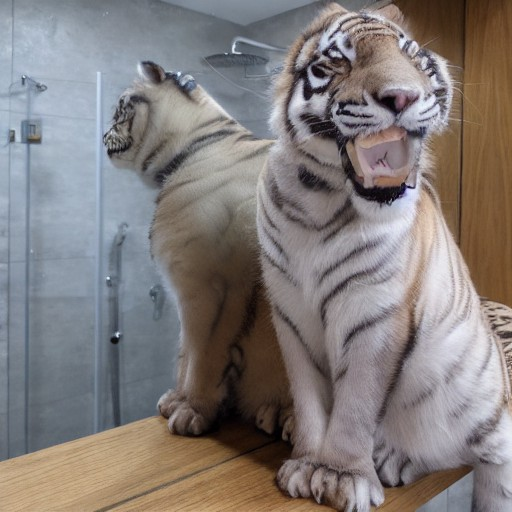
\includegraphics[width=1.5cm]{fig/cfg_self_matrix/m_2_50} & 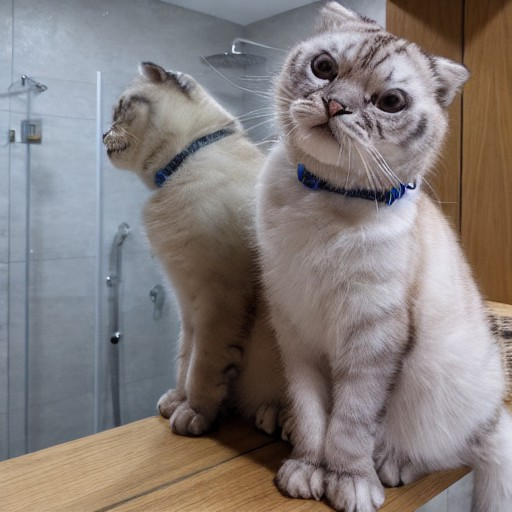
\includegraphics[width=1.5cm]{fig/cfg_self_matrix/m_2_250} & 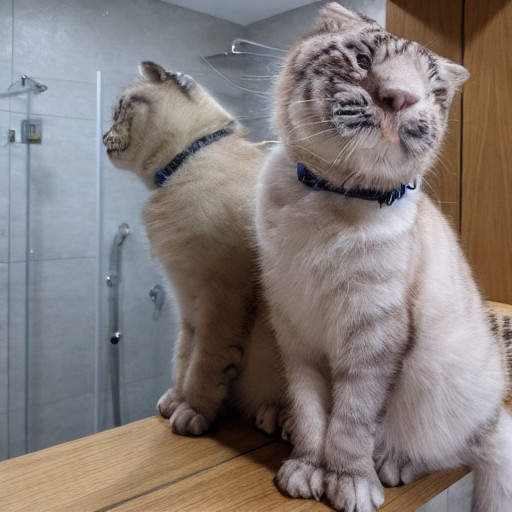
\includegraphics[width=1.5cm]{fig/cfg_self_matrix/m_2_500} & \rotatebox[origin=c]{90}{$w=2$} & \multirow{3}{*}{\rotatebox[origin=c]{90}{\textit{Classifier-Free guidance}}} \\
    
    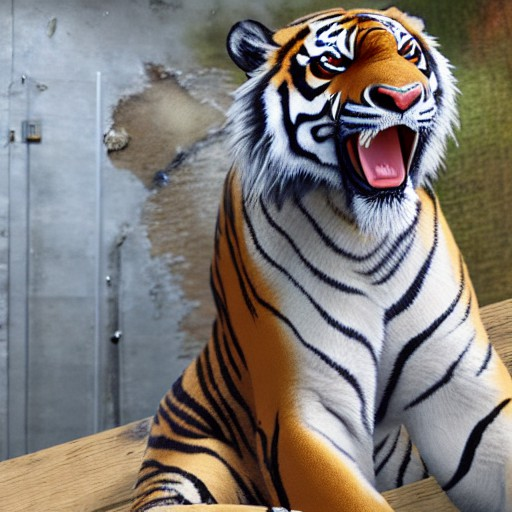
\includegraphics[width=1.5cm]{fig/cfg_self_matrix/m_75_50} & 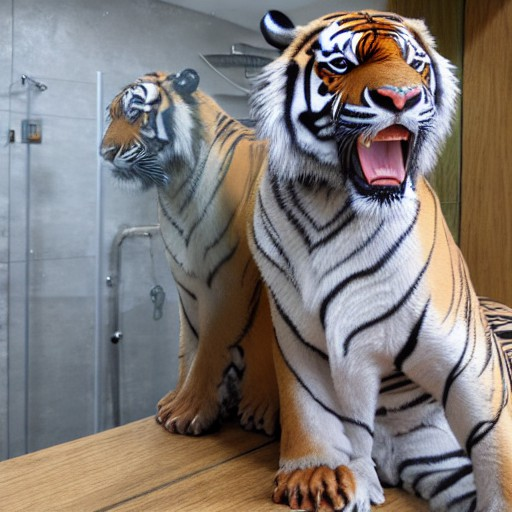
\includegraphics[width=1.5cm]{fig/cfg_self_matrix/m_75_250} & 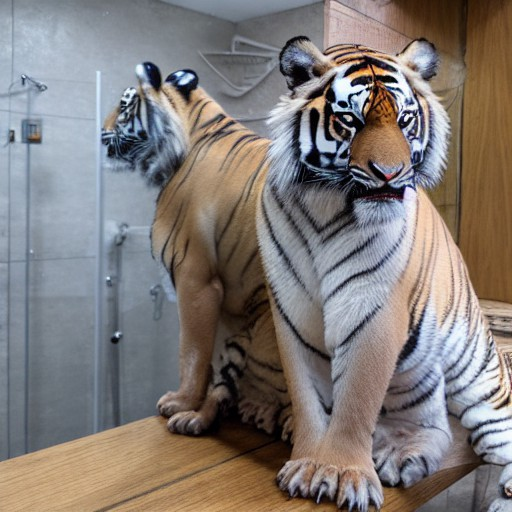
\includegraphics[width=1.5cm]{fig/cfg_self_matrix/m_75_500} & \rotatebox[origin=c]{90}{$w=7.5$} &  \\
    %   \multicolumn{7}{c}{``\textit{a baby with a stuffed \textcolor{BrickRed}{\st{monkey}} \textcolor{RoyalBlue}{\textbf{zebra}} in a car}"} \\
    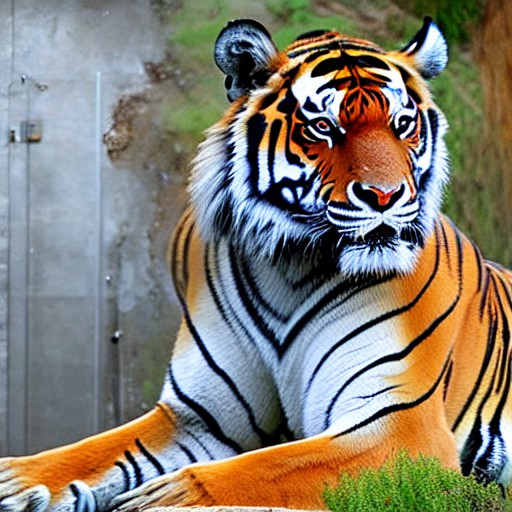
\includegraphics[width=1.5cm]{fig/cfg_self_matrix/m_15_50} & 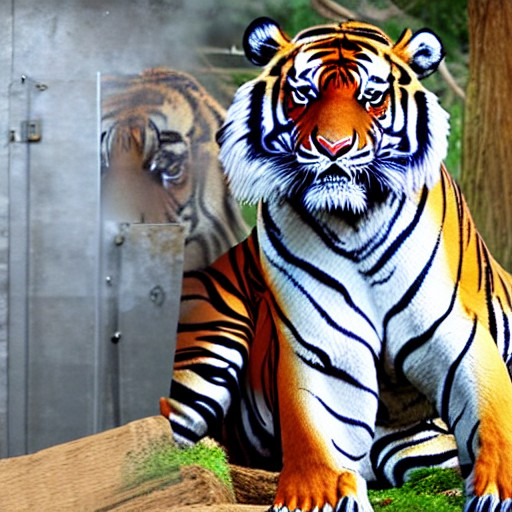
\includegraphics[width=1.5cm]{fig/cfg_self_matrix/m_15_250} & 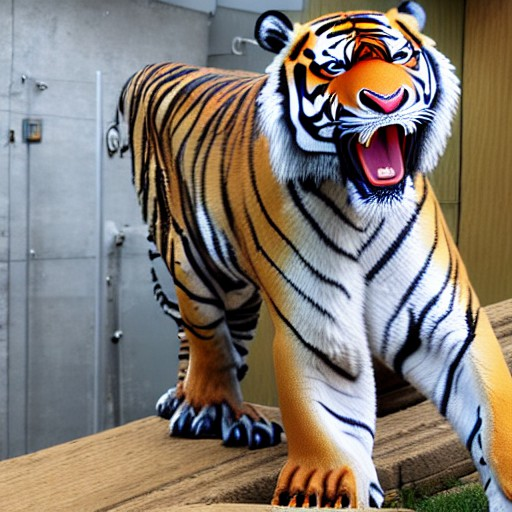
\includegraphics[width=1.5cm]{fig/cfg_self_matrix/m_15_500} & \rotatebox[origin=c]{90}{$w=15$} &  \\
    \centering  $ \lambda = 50 $  & \centering  $ \lambda = 250 $ & \centering  $ \lambda = 500 $ & & \\
    \multicolumn{3}{c}{\textit{Self-attention guidance}} & & \\
      % ... Add more rows as needed
    \end{tabular}
    % \caption{Matrix showing CFG $w$ and self-attention guidance scale $\lambda$ and how each of them drives the image generation toward reconstruction (high $\lambda$ and low $w$) or editing (low $\lambda$ and high $w$). Prompt: ``\textit{a \textcolor{BrickRed}{\st{cat}} \textcolor{RoyalBlue}{\textbf{tiger}} sitting next to a mirror}"}
    \caption{This matrix illustrates the interplay between CFG $w$ and self-attention guidance scale $\lambda$, highlighting their influence on image generation. The matrix shows how varying levels of $\lambda$ and $w$ drive the generated image toward either reconstruction (achieved with high $\lambda$ and low $w$) or editing (achieved with low $\lambda$ and high $w$). The images are generated based on the prompt ``'\textit{a \textcolor{BrickRed}{\st{cat}} \textcolor{RoyalBlue}{\textbf{tiger}} sitting next to a mirror}''.}
    \label{fig:supablation_cfg_guidance}
  \end{figure}

\subsection{Classifier-Free and Self-attention guidance} 

\label{sub:sup_results_ablation}

Figure~\ref{fig:supablation_cfg_guidance} evaluates the impact of both classifier-free guidance ($w$) and self-attention guidance ($\lambda$) on the generation process. It can be seen how a higher $\lambda$ value results in greater attention to the input structure, whereas greater $w$ values result in more plausible generation but also in more saturated colors (already discussed in \cite{ho2021classifier}). Higher self-attention guidance $\lambda$ values result in both better structure preservation and better color preservation as it reduces the negative impact of high CFG in natural looking colors. An appropiate balance is necessary to generate images that preserve the structure of the input image while performing deep, natural-looking transformations that reflect $\pout$.


\setlength{\tabcolsep}{1pt}
\begin{figure}[h]
    \footnotesize
    \small
    \centering
    % \begin{tabular}{*{6}{p{2.8cm}}}
    %   \hline
    %   & & & & & \\
    %   \centering Input & \centering \ptopzero & \centering \nulltext & \centering  \directinversion & \centering  \negprox & \centering \method{} \\
    %   %   \multicolumn{6}{c}{``\textit{A \textcolor{RoyalBlue}{\textbf{lego}} cat \textcolor{RoyalBlue}{\textbf{toy}} sitting next to a mirror}"} \\
    %   \multicolumn{6}{c}{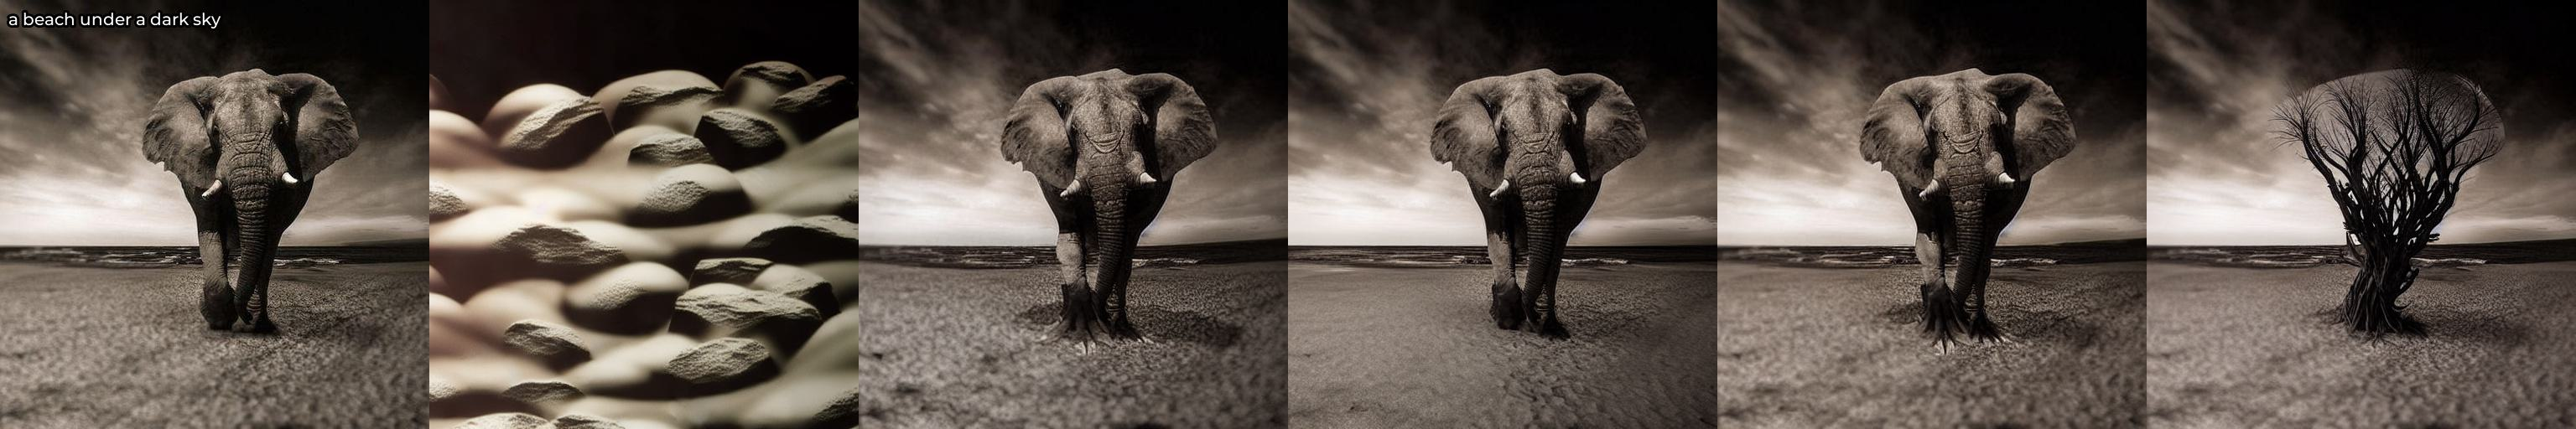
\includegraphics[width=\linewidth]{fig/ex_structpres/3_delete_object_80-2_natural-1_animal-321000000005}} \\
    % \multicolumn{6}{c}{}  \\
    % % 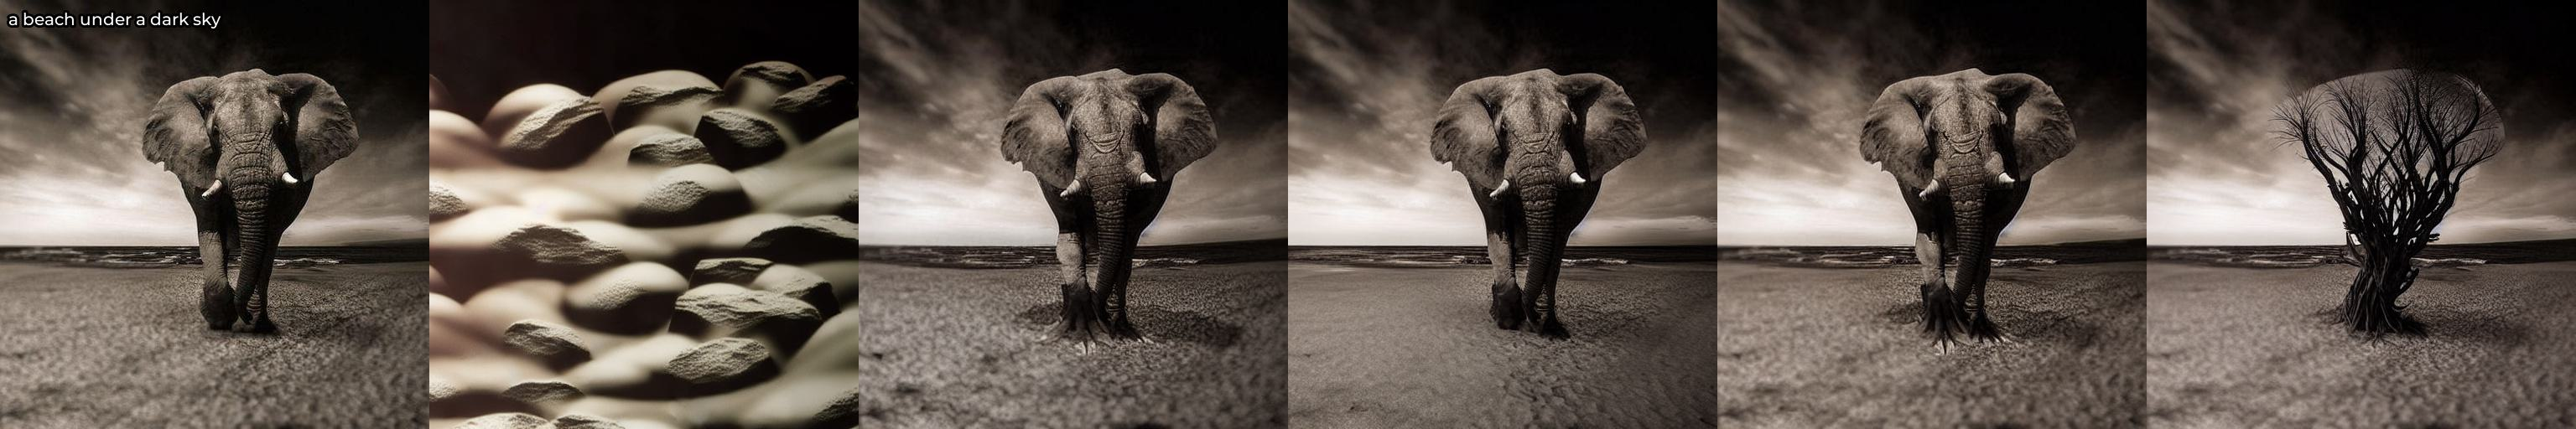
\includegraphics[height=2.2cm]{fig/ex_structpres/3_delete_object_80-2_natural-1_animal-321000000005} \\
    % %   \multicolumn{6}{c}{``\textit{Orange van with \textcolor{BrickRed}{\st{surfboards}} \textcolor{RoyalBlue}{\textbf{flowers}} on top}"} \\
    % %   \insertimage{van}{input}\\
    % %   \multicolumn{6}{c}{``\textit{Meat \textcolor{BrickRed}{\st{balls}} \textcolor{RoyalBlue}{\textbf{shushi}} on white plate}"} \\
    % %   \insertimage{meat}{input}\\
    % %   \multicolumn{6}{c}{``\textit{A \textcolor{BrickRed}{\st{woman}} \textcolor{RoyalBlue}{\textbf{storm-trooper}} with blue hair}"} \\
    % %   \insertimage{girl}{input}\\
    % %   \multicolumn{6}{c}{``\textit{A \textcolor{BrickRed}{\st{cat}} \textcolor{RoyalBlue}{\textbf{dog}} sitting on a wooden chair}"} \\
    % %   \insertimage{cat2}{input}\\
    %   \hline
    %   % ... Add more rows as needed
    % \end{tabular}
    \begin{tabularx}{0.7\columnwidth}{ YYYY }
        VAE & \method &  VAE & \method  \\
        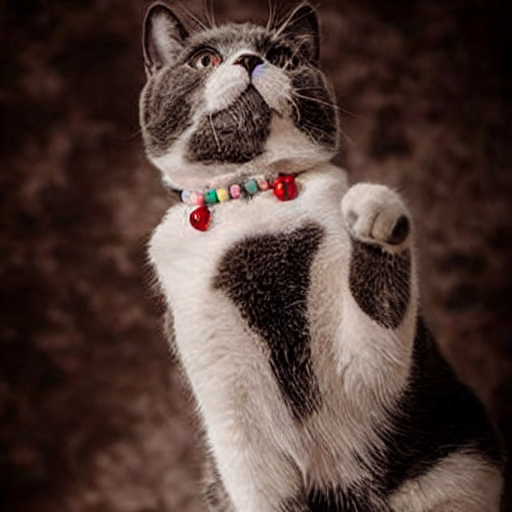
\includegraphics[width=\linewidth]{fig/reconstruction/000000000040_vae.png} & 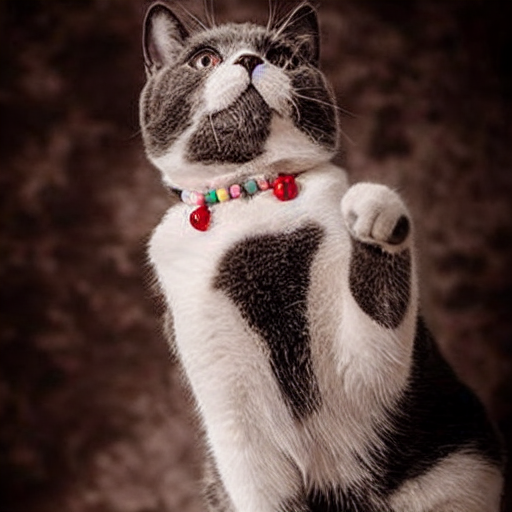
\includegraphics[width=\linewidth]{fig/reconstruction/000000000040.png} &
        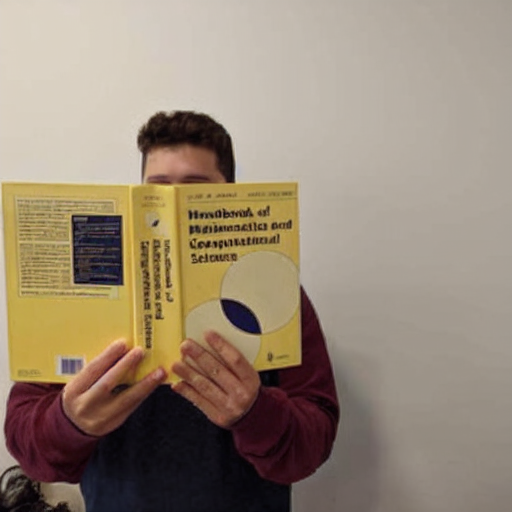
\includegraphics[width=\linewidth]{fig/reconstruction/223000000000_vae.png} & 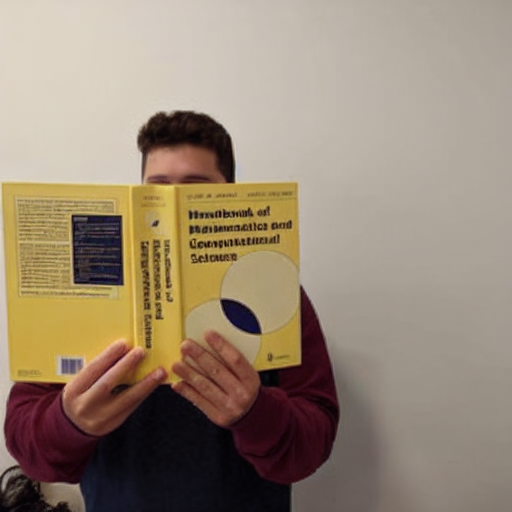
\includegraphics[width=\linewidth]{fig/reconstruction/223000000000.png}
        \\
        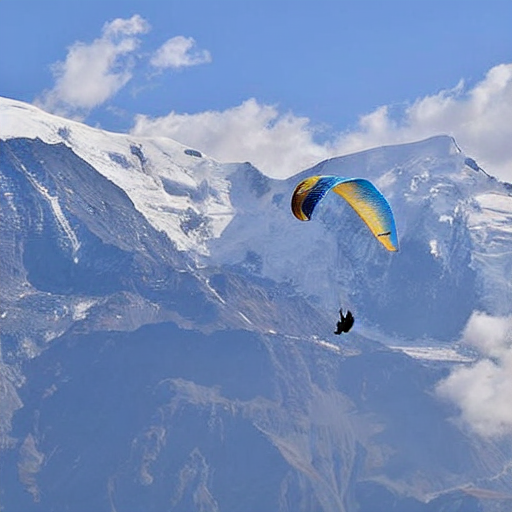
\includegraphics[width=\linewidth]{fig/reconstruction/324000000002_vae.png} & 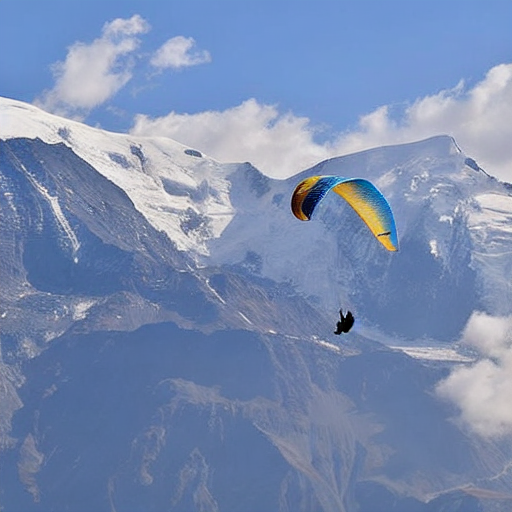
\includegraphics[width=\linewidth]{fig/reconstruction/324000000002.png} &
        
\includegraphics[width=\linewidth]{fig/reconstruction/412000000004_vae.png} & 
\includegraphics[width=\linewidth]{fig/reconstruction/412000000004.png}
        \\
        \end{tabularx}
    \caption{Reconstruction performance on PieBench samples.}
    % \caption{This figure displays examples where \method{} successfully removes objects from images, a feature not commonly observed in other negative-prompt-based methods. Each example illustrates how the removed element is replaced with content that, unexpectedly, shares structural similarities with the original object. This phenomenon, resulting from the interplay between CFG and SA guidance, highlights a unique aspect of our method's behavior and an opportunity for further refinement.} 
    \label{fig:res_reconstruction}
  \end{figure}

% \begin{table*}[htbp]
%     \centering
%       \renewcommand\arraystretch{0.9}
%       \setlength{\tabcolsep}{0.3mm}{
%     \begin{threeparttable}
%     \begin{tabular}{c|c|cccc|cc}
%     \toprule
%     \toprule
%           & \textbf{Structure}          & \multicolumn{4}{c|}{\textbf{Background Preservation}} & \multicolumn{2}{c}{\textbf{CLIP Similariy}} \\ \midrule
%     \textbf{Method}            & \textbf{Distance}$_{^{\times 10^3}}$ $\downarrow$ & \textbf{PSNR} $\uparrow$     & \textbf{LPIPS}$_{^{\times 10^3}}$ $\downarrow$  & \textbf{MSE}$_{^{\times 10^4}}$ $\downarrow$     & \textbf{SSIM}$_{^{\times 10^2}}$ $\uparrow$    & \textbf{Whole}  $\uparrow$          & \textbf{Edited}  $\uparrow$       \\ \midrule
%     \textbf{Null-text} \cite{mokady2023null} & 13.44           & 27.03  & 60.67  & 35.86  & 84.11 & 24.75        & 21.86          \\
%     \textbf{Negative prompt} \cite{miyake2023negative} &     16.17       &  26.21 &  69.01  &  39.73 & 83.40 &   24.61     &    21.87     \\
%     \textbf{Direct inversion} \cite{ju2023direct} & 11.65           & 27.22  & 54.55  & 32.86  & 84.76 & 25.02         & \textbf{22.10}          \\
%     \textbf{P2P-Zero} \cite{parmar2023zero} & 61.68 & 20.44  & 172.22 & 144.12 & 74.67 & 22.80 & 20.54 \\
%     \textbf{Plug-n-Play} \cite{tumanyan2023plug} \tnote{a} & 28.22 & 22.28  & 113.46 & 83.64 & 79.05 & 25.41 & 22.55 \\
%     \textbf{NegProx} \cite{miyake2023negative} \tnote{b} & \textbf{7.44} & \textbf{28.67} &	41.98 &	\textbf{24.25} &	\textbf{85.98} &	24.28 &	21.36 \\
%     % \textbf{Ours} (temporal) & 24.21 &	25.53 &	62.64 &	55.27 &	83.97 &	\textbf{26.18} &	\textbf{22.86} \\
%     \textbf{Ours} & 10.96 &	27.91 &	\textbf{39.56} &	29.80 &	85.97 &	\textbf{25.47} &	21.96 \\
%     \textbf{Ours} (by task) & 12.70 &	27.67 &	42.30 &	32.09 &	85.71 &	25.75 &	22.37 \\
    
%     \bottomrule
%     \bottomrule
%     \end{tabular}
%     \begin{tablenotes}
%        \footnotesize
%        \item[a] use Stable Diffusion v1.5 as base model (others all use Stable Diffusion v1.4) %revise the source code's 1000 steps to 50 steps
%        \item[b] Proximal guidance with negative prompt as introduced in \cite{han2023proximal}
%         \end{tablenotes}
%     \end{threeparttable}
%     }
%         \vspace{-0.2cm}
%     \caption{Quantitutive analysis performed on PieBench \cite{ju2023direct}. All rows but ours are taken from \cite{ju2023direct}.}
%             \label{tab:comparison_piebench}
%         \vspace{-0.2cm}
%     \end{table*}
    

% \begin{table*}[htbp]
%     \centering
%     \small
%       \renewcommand\arraystretch{0.9}
%       \setlength{\tabcolsep}{0.3mm}{
%     \begin{threeparttable}
%     \begin{tabular}{cccccc}
%    % \toprule
%     \toprule
%           & \textbf{Struct.}          & \multicolumn{2}{c|}{\textbf{Background Preservation}} & \multicolumn{2}{c}{\textbf{CLIP Similariy}} \\ \midrule
%     \textbf{Method}            & \textbf{Distance}$_{^{\times 10^3}}$ $\downarrow$ &   \textbf{LPIPS}$_{^{\times 10^3}}$ $\downarrow$  & \textbf{SSIM}$_{^{\times 10^2}}$ $\uparrow$    & \textbf{Whole}  $\uparrow$          & \textbf{Edited}  $\uparrow$       \\ \midrule
%     \textbf{\nulltextlong} \cite{mokady2023null} & 13.4             & 60.7    & 84.1 & 24.8        & 21.9          \\
%     \textbf{Negative prompt} \cite{miyake2023negative} &     16.2        &  69.0   & 83.4 &   24.6     &    21.9     \\
%     \textbf{\directinversionlong} \cite{ju2023direct} & 11.7             & 54.6    & 84.8 & 25.0         & 22.1          \\
%     \textbf{\ptopzerolong} \cite{parmar2023zero} & 61.7   & 172.2 & 74.7 & 22.8 & 20.5 \\
%     \textbf{\pnplong} \cite{tumanyan2023plug} \tnote{a} & 28.2   & 113.5 & 79.0 & 25.4 & \textbf{22.6} \\
%     \textbf{\negproxlong} \cite{miyake2023negative} \tnote{b} & \textbf{7.4}  &	42.0  &	\textbf{86.0} &	24.3 &	21.4 \\
%     % \textbf{Ours} (temporal) & 24.21 &	25.53 &	62.64 &	55.27 &	83.97 &	\textbf{26.18} &	\textbf{22.86} \\
%     \textbf{\method} (ours) & 11.0 &	\textbf{39.6} &	\textbf{86.0} &	\textbf{25.5} &	22.0 \\
%     % \textbf{Ours} (by task) & 12.70 &	42.30  &	85.71 &	25.75 &	22.37 \\
    
%     \bottomrule
%     %\bottomrule
%     \end{tabular}
%     \begin{tablenotes}
%        \footnotesize
%        \item[a] use Stable Diffusion v1.5 as base model (others all use Stable Diffusion v1.4) %revise the source code's 1000 steps to 50 steps
%        \item[b] Proximal guidance with negative prompt as introduced in \cite{han2023proximal}
%         \end{tablenotes}
%     \end{threeparttable}
%     }
%         \vspace{-0.2cm}
%     \caption{Quantitative analysis performed on PieBench \cite{ju2023direct}. All rows but ours are taken from \cite{ju2023direct}.}
%             \label{tab:comparison_piebench}
%         \vspace{-0.2cm}
%     \end{table*}




    \begin{table}[htbp]
        
    \centering
    \small
      \renewcommand\arraystretch{0.9}
      \setlength{\tabcolsep}{0.5mm}{
  \resizebox{\linewidth}{!}{  \begin{tabular}{cccccc}
   % \toprule
    \toprule
        %   & \multicolumn{4}{c}{\textbf{Structure}} & \textbf{CLIP Similariy} \\ \midrule
    \textbf{Method}            & \textbf{Struc. dist.} $\downarrow$ &   \textbf{PSNR} $\uparrow$  & \textbf{LPIPS} $\downarrow$    & \textbf{MSE}  $\downarrow$          & \textbf{SSIM}  $\uparrow$       \\ \midrule
    \textbf{VAE reconstruction} & \textbf{2.8} & \textbf{27.2} & \textbf{40.2} & \textbf{28.5} & \textbf{79.8} \\
    \textbf{\directinversionlong} \cite{ju2023direct} & 3.0 & 27.1 & 51.7 & 28.9 & 79.5\\
    \textbf{\nulltextlong} \cite{parmar2023zero} & 3.3 & 26.7 & 54.8 & 31.1 & 78.9 \\
    \textbf{\method} (ours) & 12.0 & 24.7 & 65.8 & 65.1 & 77.47\\
    
    \bottomrule
    %\bottomrule
    \end{tabular}}

    }
        % \vspace{-0.2cm}
    \caption{
        Performance of different models on PieBench samples, specifically evaluating reconstruction quality only ($\pin$ and $\pout$ are the same).
    }
            
            \label{tab:res_reconstruction}
        % \vspace{-0.2cm}
    \end{table}


  


\subsection{Self-attention guidance for reconstruction}
\label{sec:sup_reconstruction}
% In Fig \ref{fig:res_reconstruction} we compare SAGE's reconstruction performance when using the same input and editing prompt to the bare VAE reconstruction. In this evaluation, no local blending or other auxiliary techniques are applied, only self-attention guidance. The results demonstrate that SAGE can faithfully reconstruct fine details, despite not explicitly optimizing for reconstruction as \nulltextlong{} or accounting for the VAE reconstruction error as \directinversionlong{} methods do. Quantitatively, our method performs worse than these baselines in strict reconstruction metrics (see Table \ref{tab:res_reconstruction}), as they directly target the VAE latent space. However, this difference has no noticeable impact on the final editing quality, as it could be assessed in Tables \ref{tab:comparison_piebench}, \ref{tab:comparison_magicbrush} and \ref{tab:user_study} where \method{} outperform the compared methods, particularly on the reconstruction metrics.
Figure~\ref{fig:res_reconstruction} compares the reconstruction performance of \method{} given the same input image and editing prompt against the baseline VAE reconstruction. This evaluation applies only self-attention guidance, without local blending or auxiliary techniques. The results clearly show that SAGE preserves fine details despite not explicitly optimizing for reconstruction like \nulltextlong{} or compensating for VAE reconstruction errors as \directinversionlong{} does. Although our method performs worse on strict reconstruction metrics (Table~\ref{tab:res_reconstruction}) due to its indirect approach, this has no noticeable impact on final editing quality. As shown in Tables~\ref{tab:comparison_piebench}, \ref{tab:comparison_magicbrush}, and \ref{tab:user_study}, the proposed method outperforms the compared methods, particularly in reconstruction-related evaluations.





% \subsection{PieBench Examples}
% \label{sec:sup_results_piebench}

% \input{fig/ex_all1.tex}
% % \input{fig/ex_all2.tex}

% In Figure \ref{fig:sup_exall1} we show additional qualitative examples of the results corresponding to the images generated with the complete SAGE method variant \textit{(vi)} (see Table \ref{tab:ablation_piebench} of the main paper) and used for computing the metrics in Tables \ref{tab:ablation_piebench}, \ref{tab:comparison_piebench}, and \ref{tab:user_study} of the main manuscript. Our understanding is that as the self-attention maps mostly encode low-resolution semantic features instead of shapes, SAGE is able to generate images that better capture the style while changing the content (as the fox in the second row of Fig~\ref{fig:sup_exall1}), has more freedom to edit the shape of elements (as the tulips in the third row of Fig~\ref{fig:sup_exall1}), and is able to eliminate elements that are present in the original image while filling the gap with plausible content (as the camera in the last row of Figs~\ref{fig:sup_exall1} and~\ref{fig:sup_structpres}). Similarly, SAGE is the only method capable of applying pixel-art style (clown in Fig~\ref{fig:sup_exall1}). Further confirmation of our hypothesis that self-attention maps encode low-resolution semantic features is provided by the fact that SAGE changes not only the style of the last row of Fig~\ref{fig:sup_exall1} but also substantially changes the kind of chair (from modern to classic) to better fit the style of the new prompt.

% \subsection{Direct Inversion comparison}
% \label{sec:sup_results_di}

% Discuss the results of the direct inversion comparison and include the discussion with the time/mem fp16 analysis. \ref{fig:sup_ex_di_comp}.
% \directinversion{} exhibits competitive performance compared to \method{}, both in quantitative metrics and user evaluations. However, \directinversion{} struggles in specific scenarios due to its approach to content preservation through $\vz$-space reconstruction. \directinversion's performance is bound to reconstruction of the input image in the high-resolution latent $\vz$-space, which, while effective in many contexts, falls short when deviations from the source shape are required. Unlike \directinversion{}, \method{} operates on self-attention maps within a semantically-rich, lower-resolution space, affording it superior adaptability in situations where pixel-perfect accuracy is detrimental. For instance, \directinversion's limitations become evident when attempting pixel-art style transformations (as shown in Figure \ref{fig:sup_exall1}), where its inherent constraints on divergence hinder the editing of the target image style. Similarly, Figure \ref{fig:sup_ex_di_comp} highlights DI's inadequacies in image edits involving significant shape alterations or object removal, where its reliance on close adherence to the input image's structural integrity limits effective modifications.

% Even though the simpler \textit{three-code-lines} approach of DI \cite{ju2023direct} grants it a slight edge in computational efficiency, \method{}'s superior adaptability and flexibility in image editing scenarios, as well as its competitive performance in time and memory consumption, position it as a more versatile and effective solution for prompt-guided image editing.

% \input{fig/ex_di_comp.tex}

% \newpage
% \input{fig/selfreplace_fig.tex}
% \subsection{Ablation Analysis}
% \label{sec:sup_results_ablation}

% \paragraph{Self-attention replace} In Figures \ref{fig:supablation_selfreplace} we show the results of replacing the self-attention (as in \cite{hertz2023prompt}) instead of guiding the reconstruction towards them as described in Sec~\ref{sec:self_attention_guidance}. CFG $w$ values between $0$ (only $\pin$) and $1$ (only $\pout$) are able to generate plausible interpolation between both but with really poor prompt fidelity (as expected), whereas for $w$ values higher than 1, the generation quality is really poor, with oversaturated colors and artifacts. This is most likely due to the fact that direction of the second added of Eq~\ref{eq:cfg} is too high as both $\pin$ and $\pout$ self-attention maps are misaligned (guidance results in a softer difference). To solve this, \cite{hertz2023prompt} replaces the self-attention maps of both $\pin$ (or $\varnothing$) and $\pout$ inducing the need of a whole reconstruction stage (see Fig~\ref{fig:related}), not only the $\pin$ branch as we do (see Fig~\ref{fig:method_diag}).


% \paragraph{CFG and Attention reweighting} 
% %In Figure \ref{fig:supablation_cfg_weight}, we show the impact of CFG (Sec \ref{sec:self_attention_guidance}) and Attention Reweighting (Sec \ref{sec:cross_attention_manipulation}) in the generation process. Both techniques are able to increase the attention to $\pout$ but their procedure and impact is different. We show how CFG achieves more natural looking result, whereas in our example attention reweighting results in dog-features leaking to the goat. In our experience, attention reweighting should be reserved to situations where further increasing the CFG would result in unnatural results and oversaturated colors or artifacts as it usually yields better editing. If CFG is not enough, then it is better to decrease the CFG and apply attention reweighting to increase the attention to some $\pout$ key words, otherwise unnatural-looking colors are amplified when both parameters are high.
% \input{fig/competing_terms_fig.tex}
% \input{fig/cfg_weight_matrix.tex}

% In Figure \ref{fig:supablation_competing}, we illustrate the competing and coordinated nature of self-attention guidance and the Classifier-Free guidance. In Figure \ref{fig:supablation_competing_self}, we can see how self-attention guidance works through the entire image to reconstruct the input image, whereas in Figure \ref{fig:supablation_competing_cfg}, we can see how Classifier-Free guidance works only in the areas corresponding to semantic editing.

\section{Limitations}
\subsection{Structure Preservation}
\label{sec:sup_limitations_structure}


    Figure~\ref{fig:sup_structpres} shows that when objects are removed by omitting corresponding words from the prompt, \method{} fills the resulting gaps with content that maintains structural similarities to the removed elements. This behavior likely arises from a conflict between CFG—which pushes for object removal—and self-attention guidance—which favors preserving the original structure. Despite this unintended effect, \method{} is the only approach among those compared that actually removes objects, whereas other negative-prompt-based methods fail to do so. Future work may address this by selectively masking self-attention guidance in areas corresponding to the removed elements, similar to the local blending strategy.

\setlength{\tabcolsep}{1pt}
\begin{figure}[h]
    \footnotesize
    \small
    % \begin{tabular}{*{6}{p{2.8cm}}}
    %   \hline
    %   & & & & & \\
    %   \centering Input & \centering \ptopzero & \centering \nulltext & \centering  \directinversion & \centering  \negprox & \centering \method{} \\
    %   %   \multicolumn{6}{c}{``\textit{A \textcolor{RoyalBlue}{\textbf{lego}} cat \textcolor{RoyalBlue}{\textbf{toy}} sitting next to a mirror}"} \\
    %   \multicolumn{6}{c}{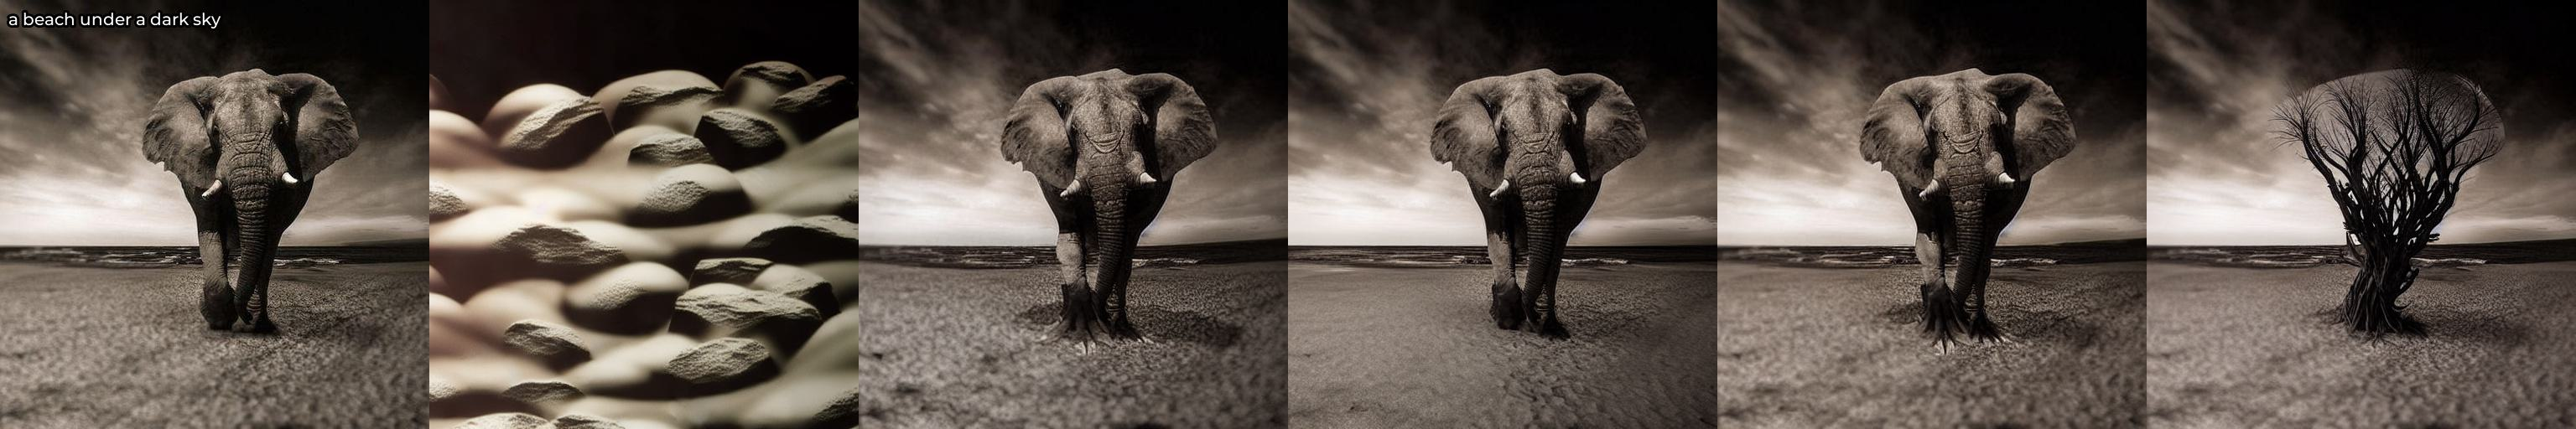
\includegraphics[width=\linewidth]{fig/ex_structpres/3_delete_object_80-2_natural-1_animal-321000000005}} \\
    % \multicolumn{6}{c}{}  \\
    % % 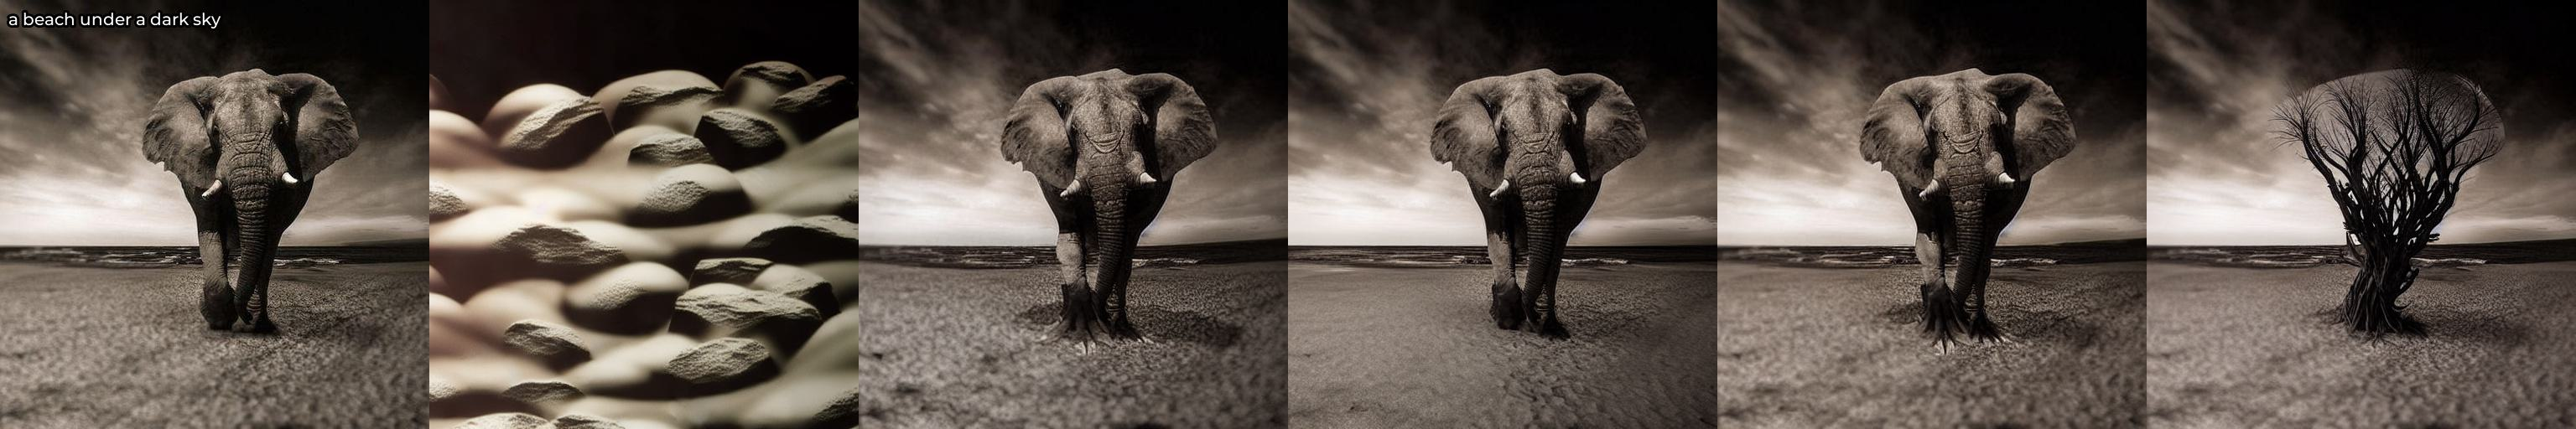
\includegraphics[height=2.2cm]{fig/ex_structpres/3_delete_object_80-2_natural-1_animal-321000000005} \\
    % %   \multicolumn{6}{c}{``\textit{Orange van with \textcolor{BrickRed}{\st{surfboards}} \textcolor{RoyalBlue}{\textbf{flowers}} on top}"} \\
    % %   \insertimage{van}{input}\\
    % %   \multicolumn{6}{c}{``\textit{Meat \textcolor{BrickRed}{\st{balls}} \textcolor{RoyalBlue}{\textbf{shushi}} on white plate}"} \\
    % %   \insertimage{meat}{input}\\
    % %   \multicolumn{6}{c}{``\textit{A \textcolor{BrickRed}{\st{woman}} \textcolor{RoyalBlue}{\textbf{storm-trooper}} with blue hair}"} \\
    % %   \insertimage{girl}{input}\\
    % %   \multicolumn{6}{c}{``\textit{A \textcolor{BrickRed}{\st{cat}} \textcolor{RoyalBlue}{\textbf{dog}} sitting on a wooden chair}"} \\
    % %   \insertimage{cat2}{input}\\
    %   \hline
    %   % ... Add more rows as needed
    % \end{tabular}
    \begin{tabularx}{\columnwidth}{ YYYYYY }
        Input & \ptopzero &  \nulltext &  \directinversion &  \negprox &  \method \\
        \multicolumn{6}{c}{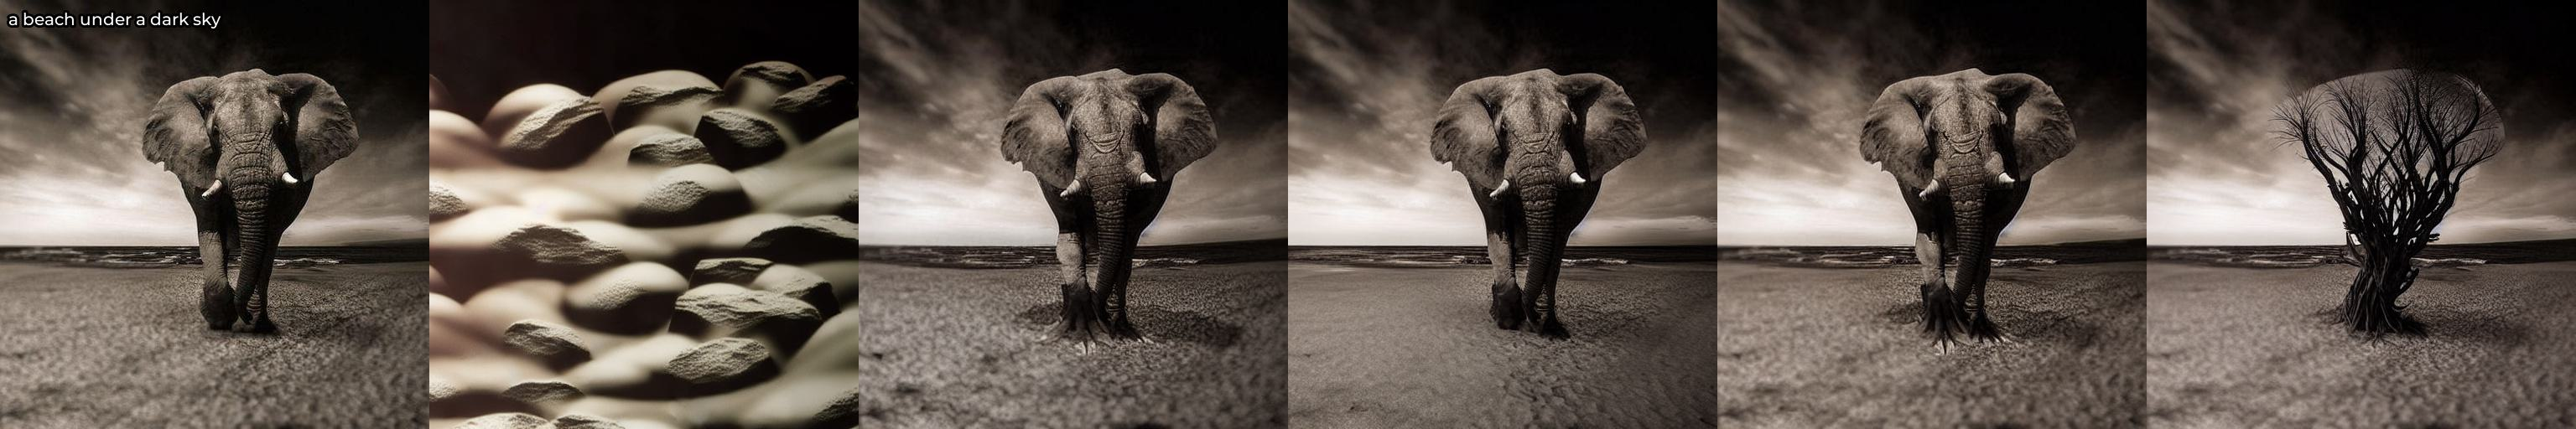
\includegraphics[width=\linewidth]{fig/ex_structpres/3_delete_object_80-2_natural-1_animal-321000000005}} \\
        \multicolumn{6}{c}{``\textit{\textcolor{BrickRed}{\st{an elephant walking on}} a beach under a dark sky}"} \\
        \multicolumn{6}{c}{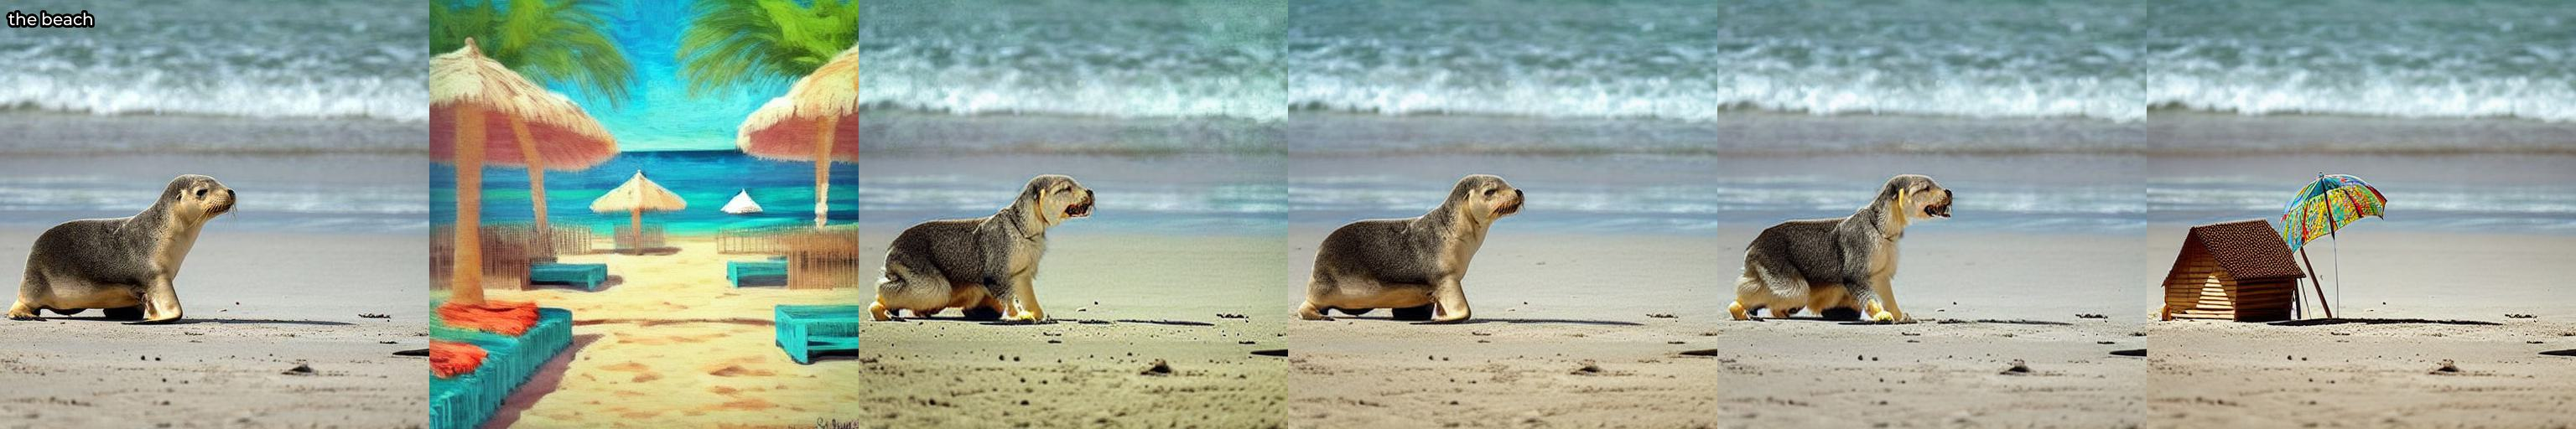
\includegraphics[width=\linewidth]{fig/ex_structpres/3_delete_object_80-2_natural-1_animal-321000000006}} \\
        \multicolumn{6}{c}{``\textit{\textcolor{BrickRed}{\st{a seal pup on}} the beach}"} \\
        
        \end{tabularx}
    % \caption{PieBench examples. STRUCTURE PRESERVATION.}
    \caption{Examples of object removal by \method{}. Although the method inadvertently fills gaps with structurally similar content, likely due to the complex interplay between CFG and self-attention guidance, it remains the only approach that consistently and effectively removes target objects.}
    \label{fig:sup_structpres}
  \end{figure}

\subsection{Failure Cases}
\label{sec:sup_limitations_failure}

\setlength{\tabcolsep}{1pt}
\begin{figure}[h]
    \footnotesize
    \begin{tabularx}{\columnwidth}{ *{6}{Y} }
        Input & \ptopzero &  \nulltext &  \directinversion &  \negprox &  \method \\
        \multicolumn{6}{c}{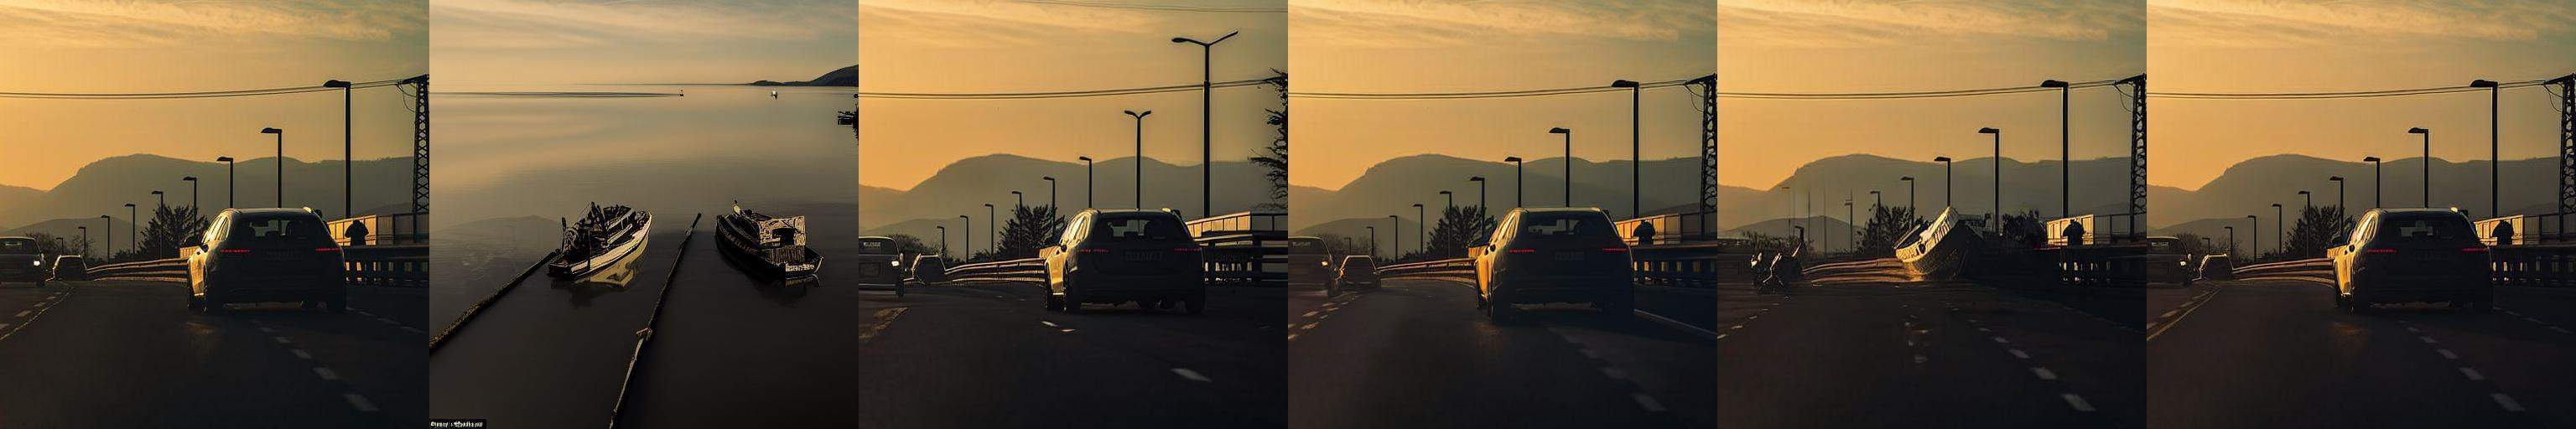
\includegraphics[width=\linewidth]{fig/ex_fail/all/1_change_object_80-2_natural-4_outdoor-124000000000}} \\
        \multicolumn{6}{c}{``\textit{\textcolor{BrickRed}{\st{cars}} \textcolor{RoyalBlue}{\textbf{boats}} driving on a highway at sunset}"} \\
        \multicolumn{6}{c}{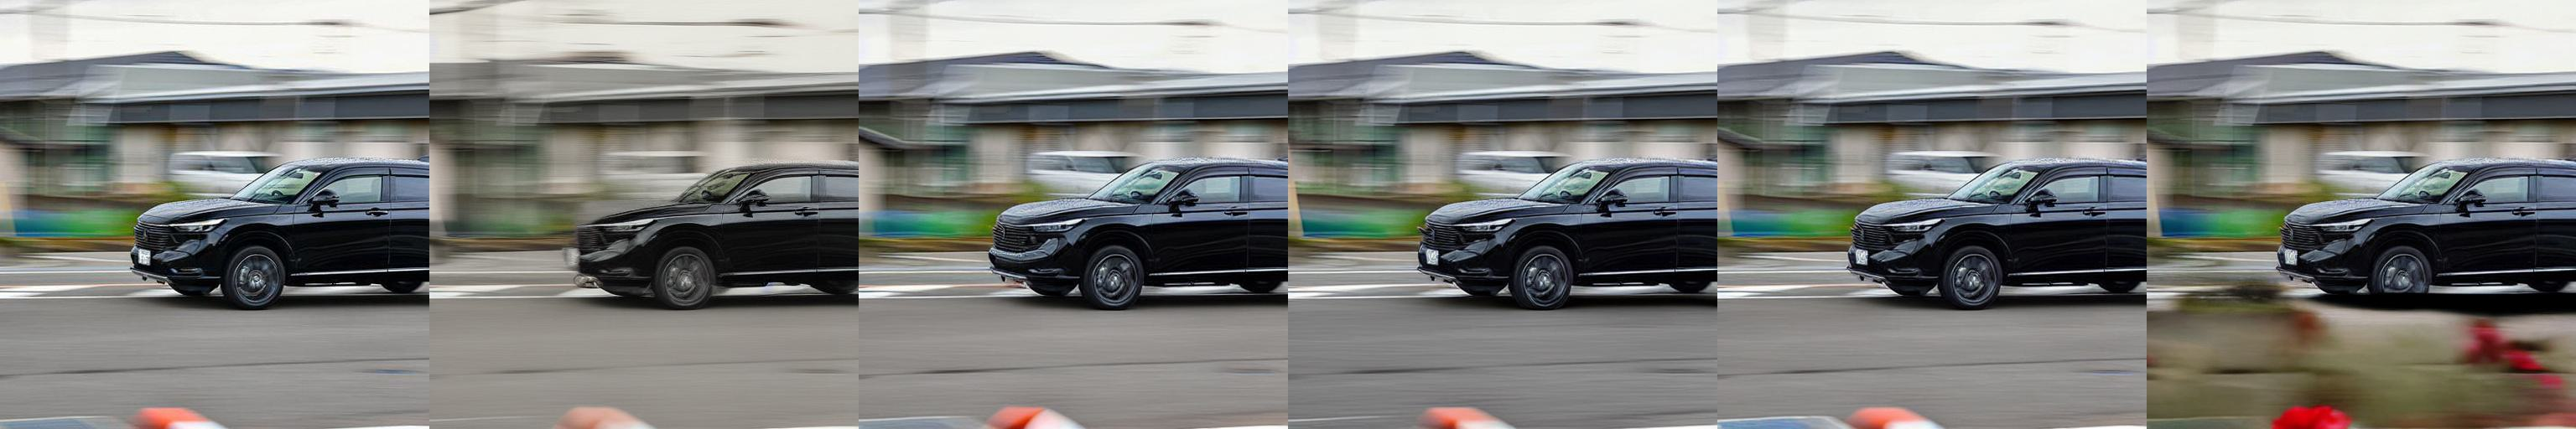
\includegraphics[width=\linewidth]{fig/ex_fail/all/7_change_attribute_material_40-2_natural-4_outdoor-724000000002}} \\
        \multicolumn{6}{c}{``\textit{the 2020 honda hrx is driving down the road \textcolor{RoyalBlue}{\textbf{full of flowers}}}"} \\
        \multicolumn{6}{c}{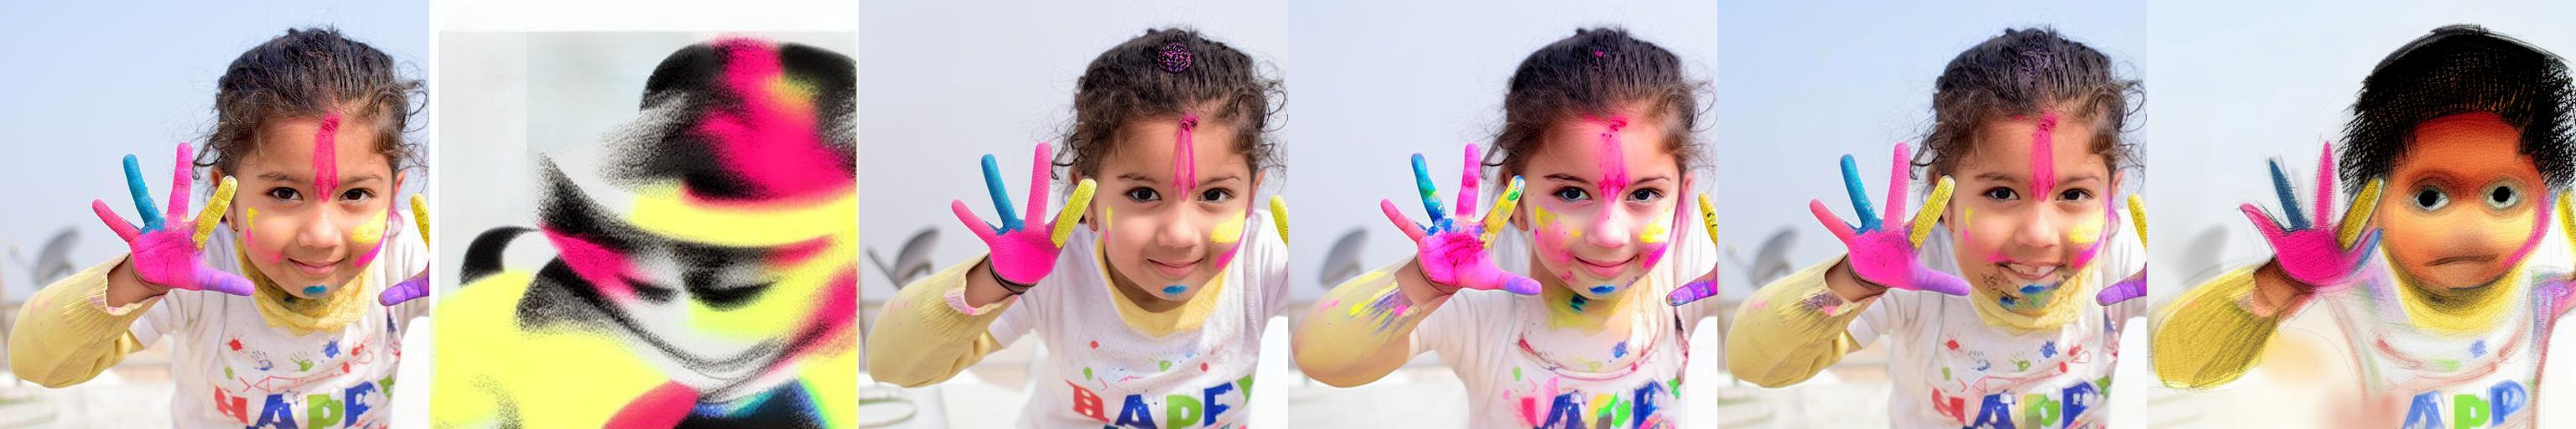
\includegraphics[width=\linewidth]{fig/ex_fail/all/9_change_style_80-2_natural-2_human-922000000009}} \\
        \multicolumn{6}{c}{``\textit{\textcolor{RoyalBlue}{\textbf{black and white sketch of}} a young girl with painted hands and face}"} \\
        \multicolumn{6}{c}{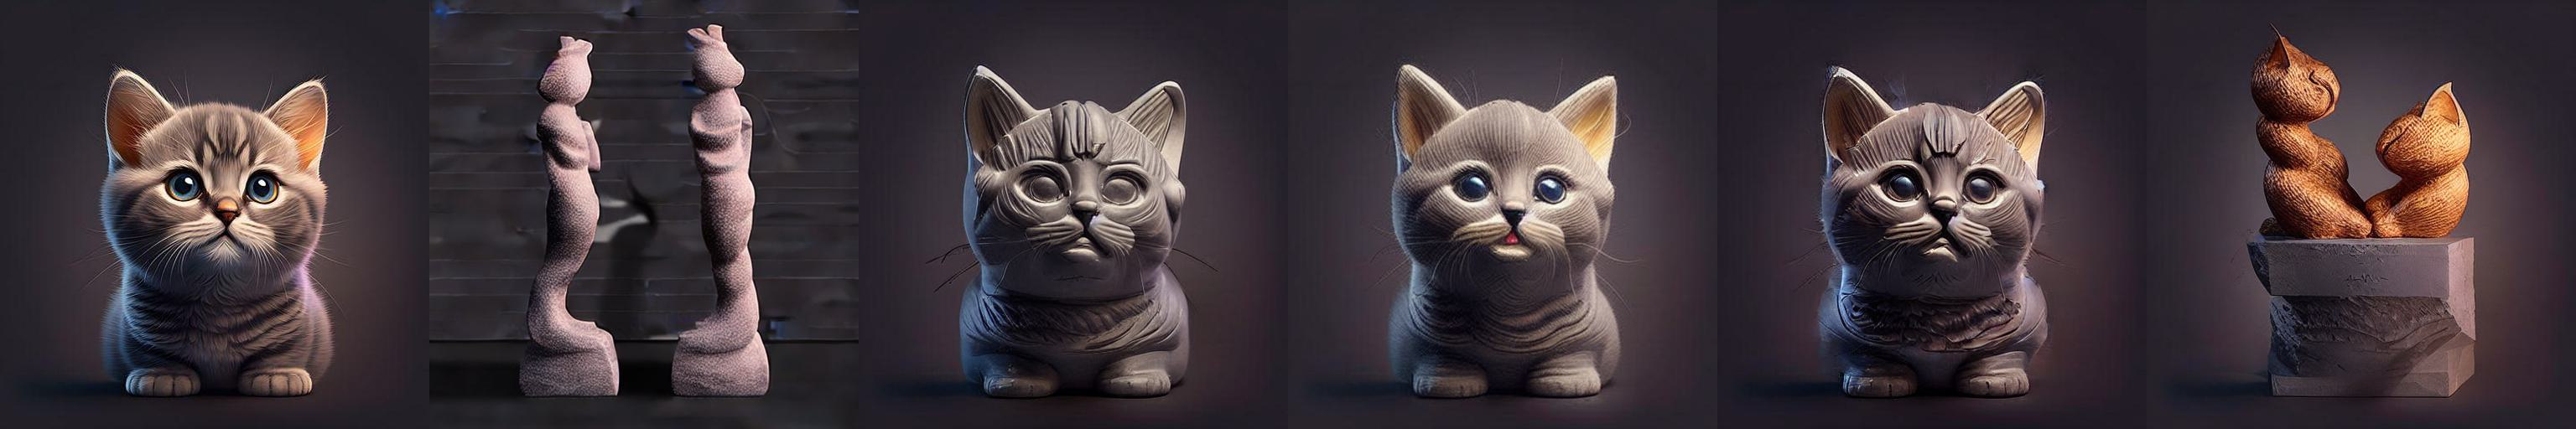
\includegraphics[width=\linewidth]{fig/ex_fail/us/7_change_attribute_material_40-1_artificial-1_animal-711000000004}} \\
        \multicolumn{6}{c}{``\textit{a kitten \textcolor{RoyalBlue}{\textbf{sculpture}} }"} \\
        \multicolumn{6}{c}{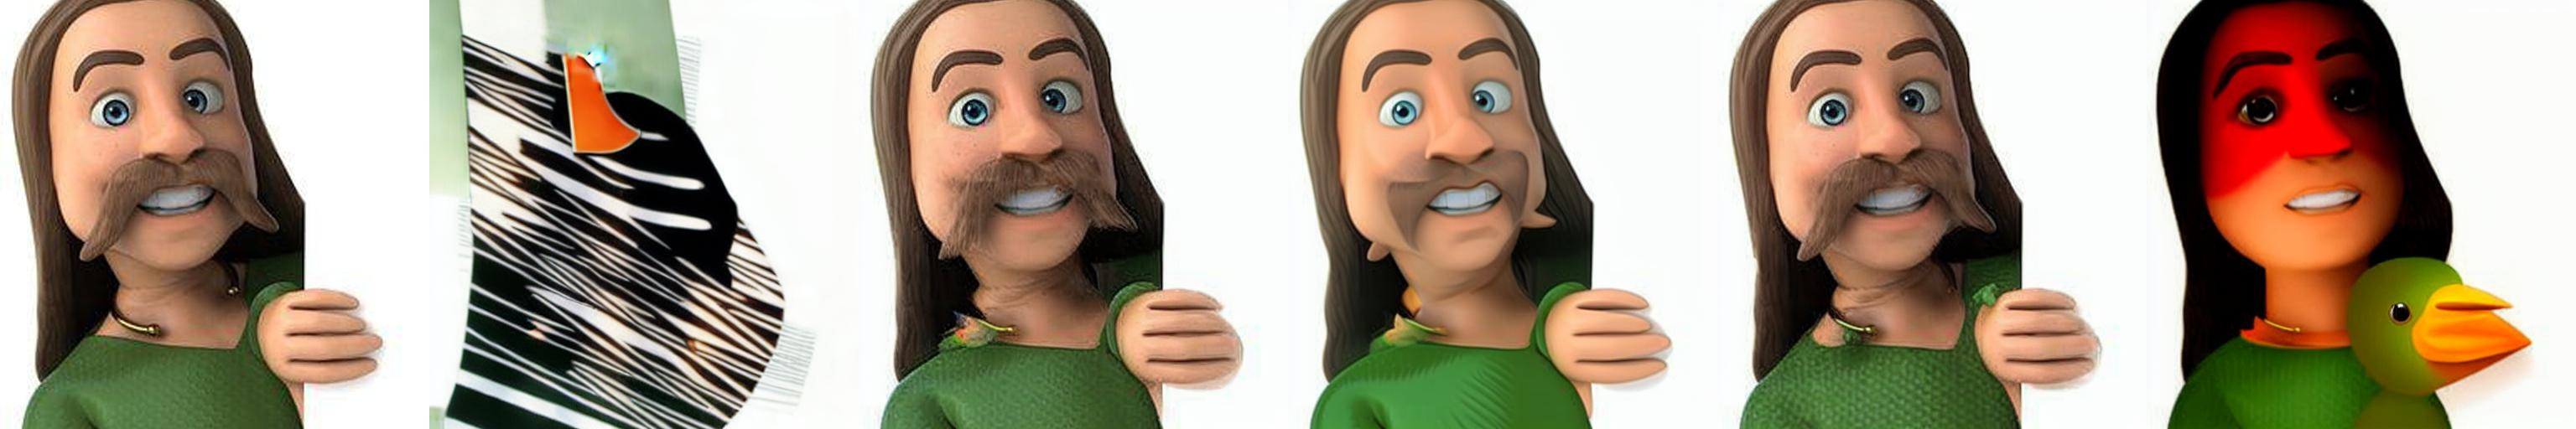
\includegraphics[width=\linewidth]{fig/ex_fail/satur/2_add_object_80-1_artificial-2_human-212000000008}} \\
        \multicolumn{6}{c}{``\textit{a cartoon man \textcolor{RoyalBlue}{\textbf{and a bird}}}"} \\
        \end{tabularx}
        \caption{This figure presents examples from the PieBench dataset where various methods, including ours, encounter difficulties in achieving the desired editing outcomes. These images highlight the challenges and limitations faced in specific editing scenarios, providing insights into areas where each method may require further refinement or adaptation.}
        % \caption{Examples from the PieBench dataset highlighting failure cases across different methods. The figure shows scenarios where the intended edits are not achieved due to the sensitivity of CFG-based approaches to hyperparameter choices. In rare instances, SAGE produces oversaturated and poorly reconstructed images—issues that can be alleviated by reducing the CFG weight ($w$) and self-attention guidance ($\lambda$).}
    \label{fig:sup_exfailall}
  \end{figure} 

% As discussed in Sections \ref{sec:limitations} of the main paper of supplementary materials, CFG-based methods are sensitive to the hyperparameters used for generation. This is specially true in the compared methods as they all include additional parameters for the editing or reconstruction. In Figure \ref{fig:sup_exfailall} we show some examples of the images corresponding to the PieBench dataset where the different methods strugle to achieve the required editing. In most of the cases, at least for SAGE, the problem can be solved by a different choice of parameters, but this is not plausible in large-scale quantitative evaluations.

% \input{fig/ex_fail_us.tex}
% In a smaller extent, we find examples where SAGE performs significantly worse than some other method. This is specially true for editings where changes are small or have fine details as \textit{spiderman} or the \textit{moon} in Figure \ref{fig:sup_exfailus}.

% \input{fig/ex_fail_satur.tex}
%Finally, we have observed that in a few cases, when all the methods fail (as happened in Fig~\ref{fig:sup_exfailall}), SAGE displays a failing behaviour different to the rest of methods. In Figure \ref{fig:sup_exfailsatur} we show some examples of this behaviour. The resulting images are oversaturated and poorly reconstructed. In these cases, the problem can be solved by reducing significantly both the CFG $w$ and Self-attention guidance $\lambda$ values.
% Finally, we have observed distinct failure patterns in SAGE, particularly in scenarios where all methods struggle. In a few cases (only 6 out of the 700 PieBench examples), SAGE tends to produce oversaturated and poorly reconstructed images, as exemplified in the last row of Fig. \ref{fig:sup_exfailall}. These issues are notably different from the failure modes of other methods. Fortunately, we found that significantly reducing both CFG $w$ and self-attention guidance $\lambda$ values can effectively address these problems, offering a viable solution for these specific failure cases.

CFG-based editing methods are inherently sensitive to hyperparameter settings, especially when additional parameters control editing or reconstruction. Figure~\ref{fig:sup_exfailall} presents examples from the PieBench dataset where various methods, including ours, struggle to achieve the intended edits. In many cases, tuning parameters can resolve the issues for SAGE, but such fine-tuning is impractical for large-scale evaluations. Notably, in a small fraction of cases (6 out of 700), SAGE produces oversaturated and poorly reconstructed images—a distinct failure mode compared to other methods. We found that significantly reducing both the CFG weight ($w$) and the self-attention guidance ($\lambda$) effectively mitigates these problems, indicating a promising direction for further refinement.
